\begin{figure}[H]
\centering
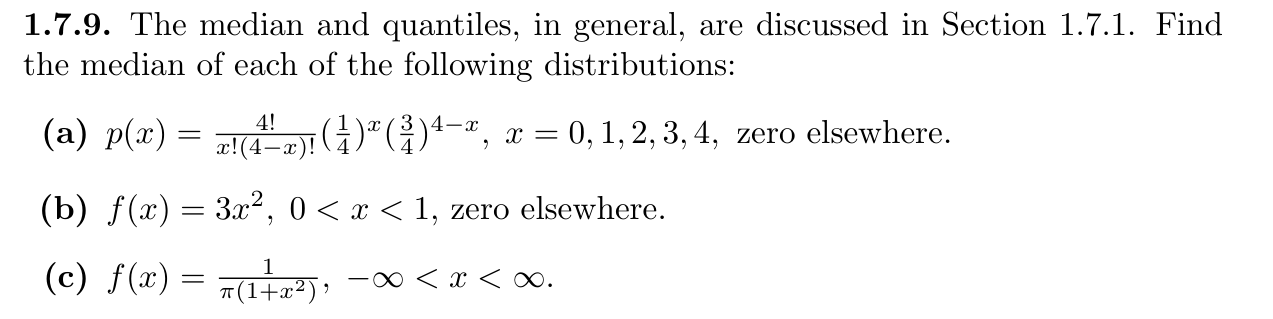
\includegraphics[width=\textwidth]{hw1-20250302.png}
% \caption{}
\label{}
\end{figure}
(a)
\[
\begin{aligned}
p(0) & =\left( \frac{3}{4} \right)^{4}=0.316406 \\
p(1) & =\left( \frac{3}{4} \right)^{3}=0.421875
\end{aligned}
\]
Then $p(x<1)\leq0.5,p(x\leq1)\geq0.5$, $\,1$ is the median. Or say that $\xi_{1/2 }\in(0,1]$.
(b)
\[
F(x)=\int_{0}^{x} 3t^{2} \, dt =t^{3}\qquad x\in(0,1)
\]
Then $\xi_{1/2 }=F^{-1}\left( \frac{1}{2} \right)=\sqrt[3]{ \frac{1}{2} }$ .
(c)
\[
F(x)=\int_{-\infty}^{x} \frac{1}{\pi(1+t^{2})}  \, dt =\frac{1}{2}+\frac{\arctan x}{\pi}
\]
Then $\xi_{1/2 }=F^{-1}\left( \frac{1}{2} \right)=0$.

\begin{figure}[H]
\centering
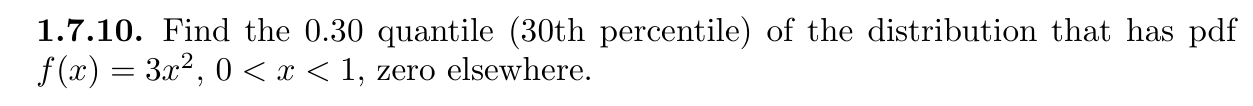
\includegraphics[width=\textwidth]{1-hw1-20250302.png}
% \caption{}
\label{}
\end{figure}
\[
F(x)=\int_{0}^{x} 3t^{2} \, dt =x^{3}\qquad x\in(0,1)
\]
Then $\xi_{0.3}=F^{-1}(0.3)=\sqrt[3]{ 0.3 }$.

\begin{figure}[H]
\centering
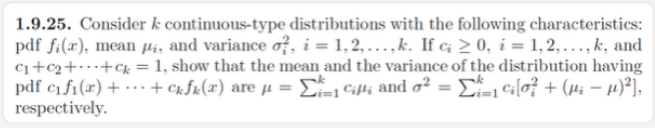
\includegraphics[width=\textwidth]{hw1-20250304.png}
% \caption{}
\label{}
\end{figure}
\[
\mu=\int_{-\infty}^{\infty} x\cdot\sum_{i=1}^{k} c_if_i(x) \, dx =\sum_{i=1}^{k} c_i\int_{-\infty}^{\infty} x\cdot f_i(x) \, dx =\sum_{i=1}^{k} c_{i}\mu _i
\]
\[
\begin{aligned}
\sigma^{2} & =\int_{-\infty}^{\infty} (x-\mu)^{2} \sum_{i=1}^{k} c_if_i(x)\, dx  \\
 & =\sum_{i=1}^{k} c_i\int_{-\infty}^{\infty} x^{2}f_i(x) \, dx -2\mu \cdot \sum_{i=1}^{k}  c_i\int_{-\infty}^{\infty} xf_i(x) \, dx +\mu^{2} \sum_{i=1}^{k} c_i\int_{-\infty}^{\infty} f_i(x) \, dx  \\
 & =\sum_{i=1}^{k} c_i\sigma _i^{2}-2\mu \cdot \sum_{i=1}^{k} c_i \mu _i +\mu^{2}\sum_{i=1}^{k} c_i \\
 & =\sum_{i=1}^{k} c_i[\sigma _i^{2}+(\mu _i-\mu)^{2}] 
\end{aligned}
\]
\begin{figure}[H]
\centering
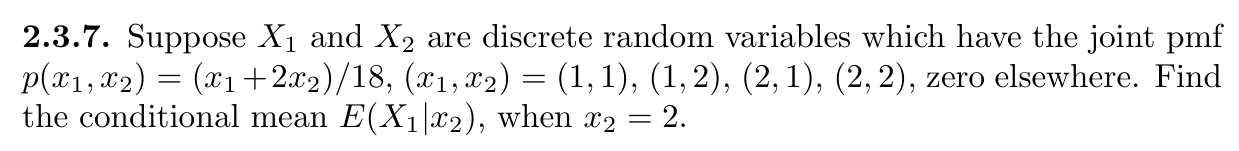
\includegraphics[width=\textwidth]{2-hw1-20250302.png}
% \caption{}
\label{}
\end{figure}
\[
\begin{aligned}
\left.E(X_{1}|x_{2})\right|_{x_{2}=2} & =\sum_{x_{1}}x_{1}\cdot \left.p_{1|2}(x_{1},x_{2})\right|_{x_{2}=2}=\sum_{x_{1}}x_{1}\cdot \left.\frac{p(x_1,x_2)}{p_2(x_2)}\right|_{x_{2}=2} \\
 & =\frac{1\cdot p(1,2)+2\cdot p(2,2)}{p(1,2)+p(2,2)}=\frac{\frac{5}{18}+2\cdot\frac{6}{18}  }{\frac{5}{18}+\frac{6}{18}  }=\frac{17}{11} 
\end{aligned}
\]
\begin{figure}[H]
\centering
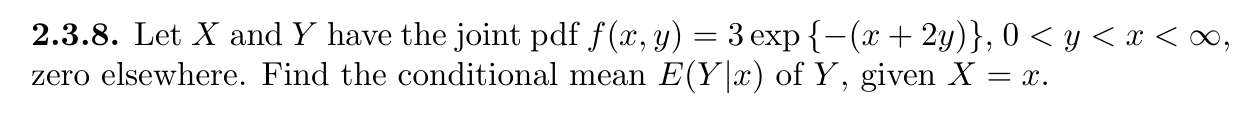
\includegraphics[width=\textwidth]{3-hw1-20250302.png}
% \caption{}
\label{}
\end{figure}
\[
\begin{aligned}
E(Y|x) & =\int_{-\infty}^{\infty} y\cdot f_{Y|X}(x,y) \, dy =\int_{-\infty}^{\infty} y\cdot\frac{f(x,y)}{f_{X}(x)} \, dy=\int_{-\infty}^{\infty} y\cdot\frac{3\exp \{ -x-2y \}\mathbb{1}_{0<y<x<\infty}}{\int_{-\infty}^{\infty} 3\exp \{ -x-2y \}\mathbb{1}_{0<y<x<\infty} \, dy } \, dy  \\
 & =\int_{0}^{x} y\cdot\frac{\exp \{ -x-2y \}}{\int_{0}^{x} \exp \{ -x-2y \} \, dy } \, dy=\int_{0}^{x} y \cdot\frac{e^{ -x-2y }}{e^{ -x }(1-e^{ -2x })/2}\, dy=\frac{2}{1-e^{ -2x }}\int_{0}^{x} y\cdot e^{ -2y } \, dy  \\
 & =\frac{e^{ 2x }-2x-1}{2(e^{ 2x }-1)} \end{aligned} 
\]
\begin{figure}[H]
\centering
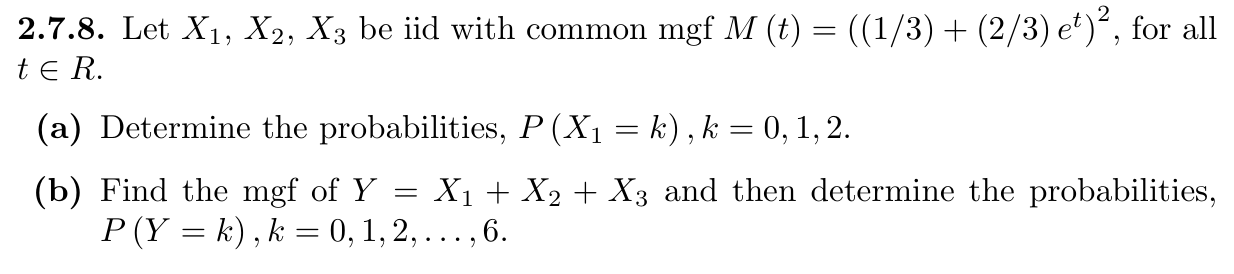
\includegraphics[width=\textwidth]{4-hw1-20250302.png}
% \caption{}
\label{}
\end{figure}

Characteristic function $\phi(t)=M(it)=\left( \frac{1}{3}+\frac{2}{3}e^{ it } \right)^{2}=\frac{1}{9}+\frac{4}{9}e^{ it }+\frac{4}{9}e^{ 2it }$, by the inverse formula
\[
f(x)=\frac{1}{2\pi}\int_{-\infty}^{\infty} e^{ -itx }\phi (t)  \, dt=\frac{1}{2\pi}\int_{-\infty}^{\infty} \frac{1}{9}e^{ -itx }+\frac{4}{9}e^{ -it(x-1) }+\frac{4}{9}e^{ -it(x-2) } \, dt = \frac{1}{9}\delta_0+\frac{4}{9}\delta_1+\frac{4}{9}\delta_2
\]
Then $X_1$ is discrete random variable with $P(X_1=0)=\frac{1}{9},P(X_1=1)=\frac{4}{9},P(X_1=2)=\frac{4}{9}$.
The mgf of $Y=X_1+X_2+X_3$ is
\[
M_{Y}(t)=E(e^{ t(X_1+X_2+X_3) })\overset{ iid }{ = }E(e^{ tX_1 })E(e^{ tX_2 })E(e^{ tX_3 })=\left( \frac{1}{3}+\frac{2}{3}e^{ t } \right)^{6}
\]
\begin{table}[h]
	\centering
	\begin{tabular}{|c|c|c|c|c|c|c|c|}
		\hline
		$Y$ & 0 & 1 & 2 & 3 & 4 & 5 & 6 \\
		\hline
		$P$ & $\frac{1}{729}$ & $\frac{4}{243}$ & $\frac{20}{243}$ & $\frac{160}{729}$ & $\frac{80}{243}$ & $\frac{64}{243}$ & $\frac{64}{729}$ \\
		\hline
	\end{tabular}
\end{table}